
\subsection{Implementation}
After the necessary introduction to \gls{opengl} in the previous chapter, this one is aimed at the functionality of the \emph{Jaw Viewer} and the steps encountered over the duration of this project.

\subsubsection{Import Anatomy}

The first goal of the project was loading \glspl{anatomy}. As described in \ref{uc:1} UC01: Load Anatomy, the user selects and loads the Anatomy Objects in form of \gls{STL} files. Before explaining how we import these files, we extend the \gls{gls-STL} explanations in the glossary with more information on the file structure. 


\subsubsubsection{STL file structure}

The structure of a STL file can be ASCII or binary. The \textbf{ASCII representation} of a STL file always begin with the line: 

\centerline{\texttt{solid name}}
 
\noindent where \verb|name| is an optional string. The file contains the representation of any number of triangles with its coordinates:

\begin{figure}[h!]
	\centering
	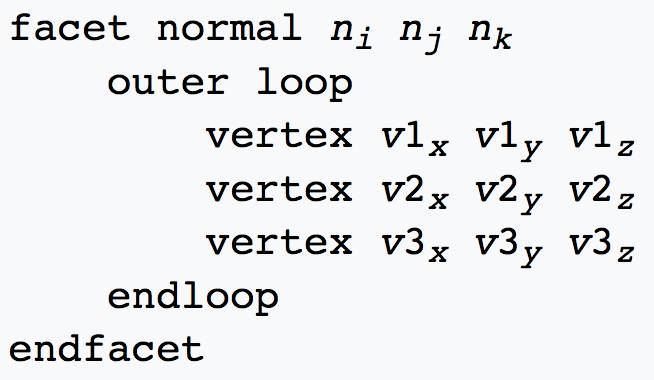
\includegraphics[width=0.25\textwidth]{stl_ascii}
	\caption{STL file Ascii representation \cite{stl-wikipedia}}
\end{figure}


\noindent The file concludes with: 

\centerline{\texttt{endsolid name}}
\bigskip


A \textbf{binary STL file} has an 80-character header. Following the header, there is a 4-byte unsigned integer indicating the number of triangular facets in the file as well as the data describing each triangle in turn. The file simply ends after the last triangle.

\noindent Each triangle is described by twelve 32-bit floating-point numbers: three for the normal and then three for the $X/Y/Z$ coordinate of each vertex. After these follows a 2-byte ("short") unsigned integer that is the "attribute byte count" \cite{stl-wikipedia}.

\begin{figure}[h!]
	\centering
	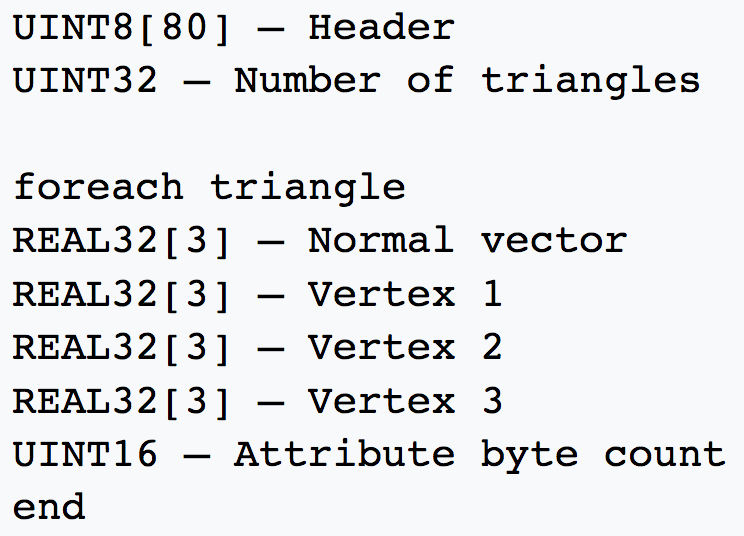
\includegraphics[width=0.25\textwidth]{stl-binary}
	\caption{STL file Binary representation \cite{stl-wikipedia}}
\end{figure}

\subsubsubsection{Importing STL files} \label{importing-stl-files}

The tutorial \cite{learnopengl} we used as base for this project employed the C++ library \verb|assimp| \cite{assimp} to import STL files. As \verb|assimp| introduced an external dependency with a lot more functionality and complexity than required by this project, we decided not to use \verb|assimp| and implement our own STL file reader instead. 

As already mentioned in \ref{architecture} architecture, the \verb|common| package contains the \verb|StlFileManager| class, responsible of parsing \gls{STL} files in ASCII and binary format.

The  \verb|StlFileManager| receives the path to the file (\verb|parse_stl_file(const std::string filePath)|), checks if the file exists and if it is binary or ASCII, parses it and returns all the \gls{vertex} data wrapped in the \verb|StlData| class:

\begin{lstlisting}[language=C++, caption=StlData]
class StlData {
	public:
	std::string name;
	std::vector<Triangle> triangles;	
	StlData(const std::string name) : name(name) { }
};
\end{lstlisting}

\subsubsection{Display Anatomy} \label{display-anatomy}

The \ref{uc:5} UC05: Display anatomy movement describes how the system displays the Anatomy objects. In order to explain how this is done, we must first go through the whole application starting process.

We assume that \ref{uc:1} UC01: Load anatomy has already taken place. This means, that the C\# GUI hat already saved all the from user entered paths to STL files and other necessary configuration parameters in a \verb|JSON| configuration file. The path to the \verb|JSON| configuration file is passed to the \verb|GameController| class. As its name indicates, this class is responsible for the management of the application and is contained in the \verb|viewer| package.

The \verb|GameController| initializes \gls{opengl}, GLEW \cite{glew}, the displayable components and loads the configuration from the \verb|JSON| file. For this, the path to the \verb|JSON| file is passed to the \verb|JsonReader|, another helper class in the \verb|common| package, which extracts the configuration data and stores it in the \verb|ConfigurationData| class. The \verb|GameController| run the \verb|GameLoop| and initializes also the \verb|UiControllers|.

The above mentioned displayable elements are exactly that: software objects or classes which represent something displayed on the screen. Among these are the \Gls{scene} and another elements like the \gls{reference-cube}, the \gls{camera-leds} and \glspl{mesh}. Being a displayable element as well, the scene contains all these elements. Once initialized, the scene initializes the Reference Cube, the Camera Leds as well as the Meshes. The meshes are displayed by means of the STL file paths saved in the \verb|ConfigurationData| class.

Slowly we get closer to the initial goal, displaying the anatomy. As described in the glossary, a \gls{mesh} is \emph{already} an anatomy object. After initializing the meshes, the \verb|mesh.loadMeshDataFromStlFile(filePath)| method is called on each mesh object. In this method the \verb|StlFileManager| class is used to get the \verb|StlData| (see \ref{importing-stl-files} Importing STL files), and finally the necessary vertices and indices are obtained from the \verb|StlData|.

\begin{lstlisting}[language=C++, caption={Loading Mesh data from Stl files}]
void Mesh::loadMeshDataFromStlFile(const std::string filePath) {
	stl::StlFileManager stlFileManager{};
	auto stlData = stlFileManager.parse_stl_file(filePath);
	this->vertices = this->getVerticesFromStlData(stlData);
	this->indices = this->getIndicesFromStlData(stlData);
}	
\end{lstlisting}
At this point in time, each Mesh has loaded all the elements to be displayed on the screen. But all these vertices and indices must be first processed by OpenGL and submitted to the graphics processing unit (GPU). These operations are executed on each Mesh object by calling the method \verb|setupMesh()|:

\begin{lstlisting}[language=C++,caption={Setting up a Mesh}]
void Mesh::setupMesh() {
	glGenVertexArrays(1, &this->VAO);
	glGenBuffers(1, &this->VBO);
	glGenBuffers(1, &this->EBO);
	glBindVertexArray(this->VAO);
	glBindBuffer(GL_ARRAY_BUFFER, this->VBO);
	glBufferData(GL_ARRAY_BUFFER, this->vertices.size() * sizeof(Vertex), 
						&this->vertices[0], GL_STATIC_DRAW);
	glBindBuffer(GL_ELEMENT_ARRAY_BUFFER, this->EBO);
	glBufferData(GL_ELEMENT_ARRAY_BUFFER, this->indices.size() * sizeof(GLuint), 
						&this->indices[0], GL_STATIC_DRAW);
	glEnableVertexAttribArray(0);
	glVertexAttribPointer(0, 3, GL_FLOAT, GL_FALSE, sizeof(Vertex), 
						static_cast<GLvoid*>(nullptr));
	glEnableVertexAttribArray(1);
	glVertexAttribPointer(1, 3, GL_FLOAT, GL_FALSE, sizeof(Vertex), 
						reinterpret_cast<GLvoid*>(offsetof(Vertex, Normal)));
	glBindVertexArray(0);
}
\end{lstlisting}

\noindent The last step is done in the so called \verb|{game loop}|. While running inside this loop, the \verb|Scene| calls the \verb|Draw(Shader shader)| method for each 
Mesh object, passing the necessary \verb|Shader| to it. So each Mesh object is finally displayed on the screen (figure \ref{fig:anatomy-objects}).

\begin{figure}[h!]
	\centering
	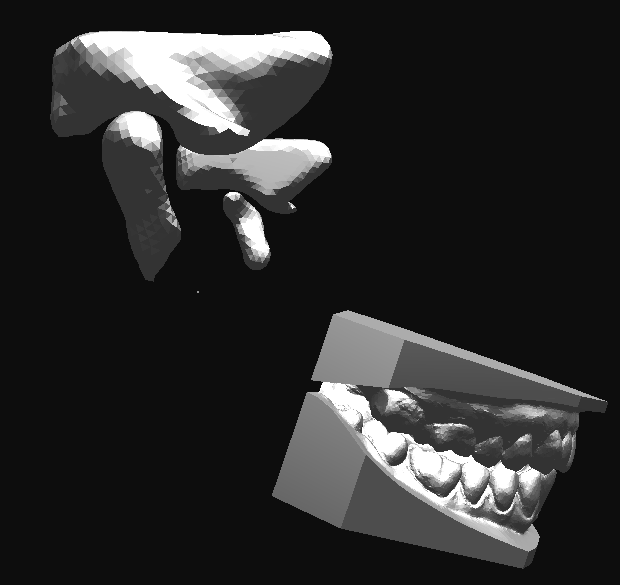
\includegraphics[width=0.35\textwidth]{jaw_viewer}
	\caption{Anatomy Objects in the \emph{Jaw Viewer}}
	\label{fig:anatomy-objects}
\end{figure}




\subsubsection{Import movement or MVM files}

The Use Case \ref{uc:2} Load movement describes how the user selects and loads the movement files or \gls{MVM} files. Once more, before going into the explanation of how the MVM files are loaded, we will describe their structure and function.


\subsubsubsection{MVM files} \label{mvm-file}

A MVM or motion movement file is a file generated by the proprietary \gls{optis} application used by the clinic. Each file contains snapshots of LED coordinates recorded by 3D cameras during jaw movement. In other words, a MVM file is a recording in coordinates of the patient's jaw movement.
The LEDs are grouped in triangles and attached to the patient's jaw. Each of the recording cameras covers one axis, making them essentially 3D, and the coordinates of each camera (X, Y, Z) on one step combined represent one \gls{frame}. In addition to the calculated coordinates, the luminosity readings from the sensors used for the detection or identification of the LED are also stored in each set of data.
\begin{figure}[h!]
	\centering
	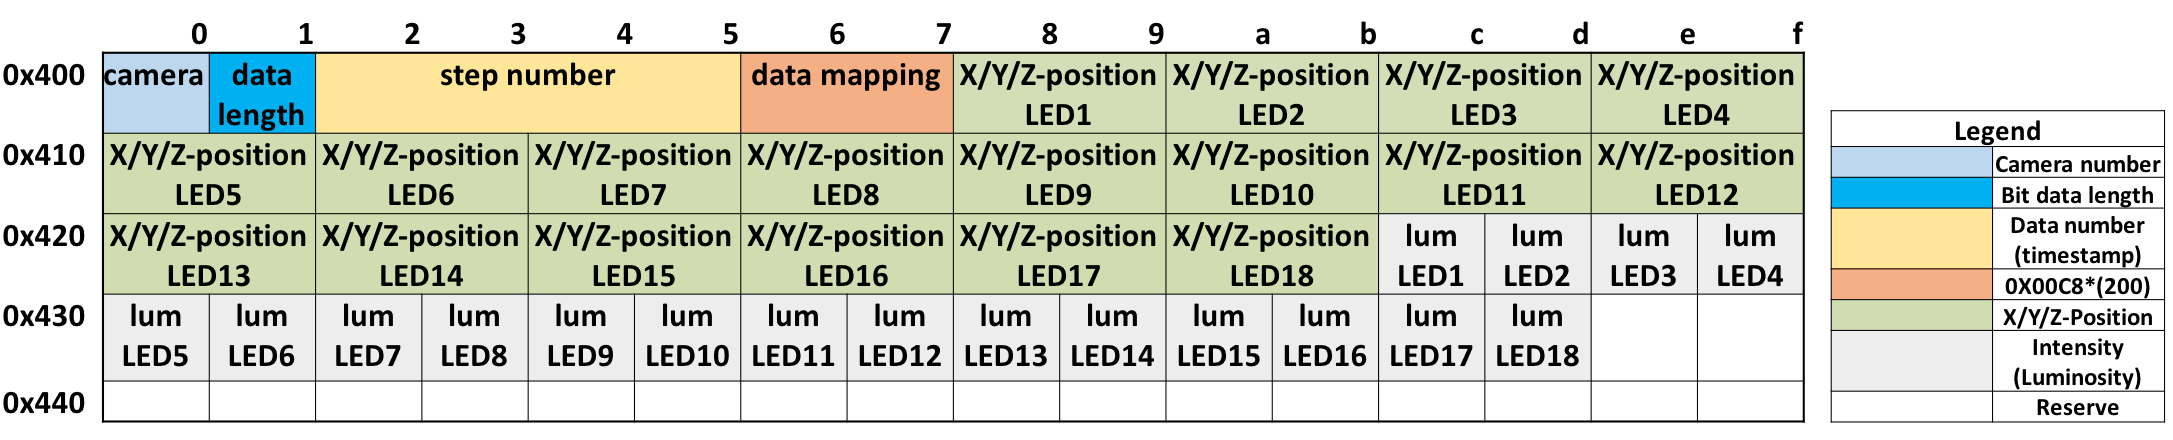
\includegraphics[width=1\textwidth]{mvm}
	\caption{MVM file structure}
	\label{fig:mvm-structure}
\end{figure}

The figure \ref{fig:mvm-structure} shows the structure of one camera. Placed after the 1024 bytes file header, the camera structure has a length of 62 bytes and contains among other data, the coordinates of each camera Led and its luminosity value. This structure is repeated until file ends.

In a MVM file these structures are grouped by three, forming a \gls{frame}, and within each frame the 18 LEDs forming triangles (f.e. LEDs 1, 3, 5 resemble a triangle). Each structure is separated from the next by an empty padding space of 194 bytes. 

The set of frames saved in a MVM file constitute a movement. You can think of the frames like the individual film frames which together compose the complete moving picture.

\begin{figure}[h!]
	\centering
	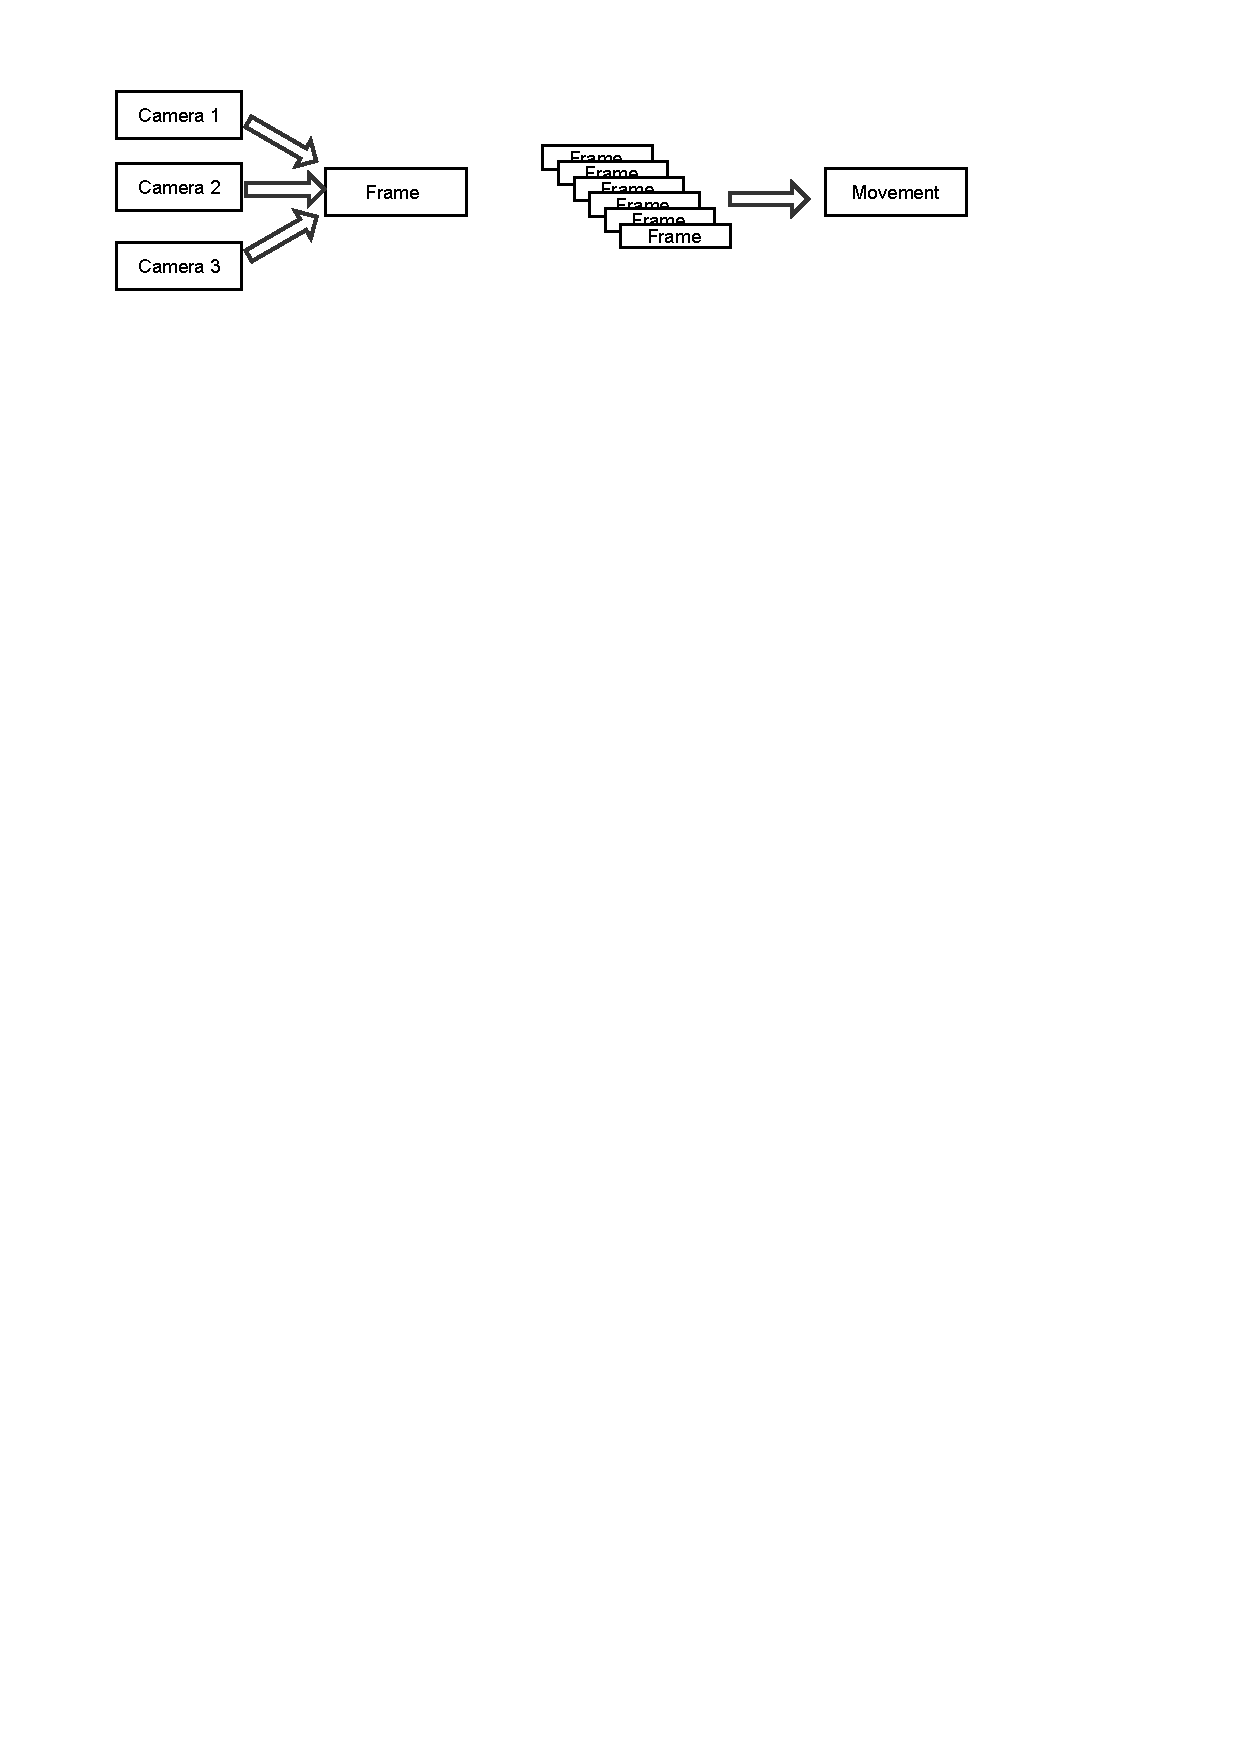
\includegraphics[width=0.6\textwidth]{ba_frames}
	\caption{Frames and Movement}
\end{figure}


\subsubsubsection{Reading MVM files} \label{reading-mvm-files}

Now to the loading or reading process. The MVM files are a proprietary format of the Clinic for Masticatory Disorders, and therefore there are no C++ libraries which support parsing them. Due to that fact, we had to implement a custom MVM file reader. The \verb|MvmFileManager| class, another helper class in the \verb|common| package, accomplishes this functionality.

\noindent The \verb|MvmFileManager| uses the \verb|MvmFileCamera| struct, which corresponds to the MVM camera structure of Figure \ref{fig:mvm-structure}:


\begin{lstlisting}[language=C++,caption={The MvmFileCamera struct},label={code:mvmfilecamera}]
struct MvmFileCamera {
	uint8_t cameraNumber{};
	uint8_t bitDataLength{};
	uint32_t stepNumber{};
	uint16_t dataMapping{};
	std::vector<uint16_t> leds;
	std::vector<GLfloat> convertedLeds;
	std::vector<uint8_t> luminosities;

	static constexpr double upperOldLevel = 65535.0;
	static constexpr double interval = 327.68;
	static constexpr double bottomNewLevel = -163.84;

	MvmFileCamera() : leds(18), convertedLeds(18), luminosities(18) {}

	/**
	* \brief Translates the given led coordinate from the in MVM file saved format 
	* (integer from 0 to 65535) to the new range (-163.84 to 163.84 millimeter)
	* \param originalCoordinate
	* \return GLfloat
	*/
	static GLfloat getCoordinateInverseMapping(const uint16_t originalCoordinate) {
		return (originalCoordinate / upperOldLevel) * (interval) + (bottomNewLevel);
	}
	
	void translateLedCoordinates() {
		std::transform(
			leds.cbegin(), 
			leds.cend(), 
			convertedLeds.begin(),
			getCoordinateInverseMapping
		);
	}
};
\end{lstlisting}

Basically, the \verb|MvmFileManager| receives the path to the \gls{MVM} file, opens it, extracts the data to \verb|MvmFileCamera| instances, processes the data in these instances and then returns the information as a collection of frames:
\begin{lstlisting}[language=C++,caption={MvmFileManager getFramesFromMvmFile method}, label={code:mvmfilemanager}]
std::vector<Frame> MvmFileManager::getFramesFromMvmFile(const std::string pathTofile) {
	std::ifstream mvm_file(pathTofile, std::ios::in | std::ios::binary);
	static_assert(CHAR_BIT == 8, "Expecting char to consist of 8 bits");
	try {
		auto fileLenght = this->getFileLength(mvm_file);
		auto fileIndex{firstFileIndex};

		while (fileIndex < fileLenght) {
			auto camera1 = this->getCameraData(mvm_file, fileIndex);
			fileIndex += fileIndexOffset;	//fileIndexOffset = 256;
			auto camera2 = this->getCameraData(mvm_file, fileIndex);
			fileIndex += fileIndexOffset;
			auto camera3 = this->getCameraData(mvm_file, fileIndex);
			fileIndex += fileIndexOffset;
			auto frame = this->getFrameFromCameradata(camera1, camera2, camera3);
			this->frames.push_back(frame);
		}
		mvm_file.close();
		return this->frames;
	} catch //... error handling
\end{lstlisting}

The \verb|MvmFileManager::getCameraData(...)| method recursively extracts the data from the \verb|ifstream| to an instance of the \verb|MvmFileCamera| struct and translates the LED coordinates.
This translation is necessary because the LED coordinates in the MVM file are saved as unsigned integers from 0 to 65535 (for the transmission protocol), and in the \emph{Jaw Viewer} the coordinates must be calculated back into their original range from -163.84 to 163.84 millimeters. The method \verb|translateLedCoordinates| in listing \ref{code:mvmfilecamera} executes this translation.

As already mentioned above, three \verb|MvmFileCamera| instances are necessary to form a frame, and the camera structures are separated by 194 empty bytes. Because of that, the method \verb|getFramesFromMvmFile| (Listing \ref{code:mvmfilemanager}) iterates through the file in "jumps" of 256 bytes until the MVM file ends.
In each of this iterations, when three \verb|MvmFileCamera| instances are ready, the method \verb|MvmFileManager::getFrameFromCameradata(camera1, camera2, camera3);| creates an instance of the \verb|Frame| class (Listing \ref{code:frame}) and saves it in a \verb|std::vector|.

\begin{lstlisting}[language=C++,caption={Frame class}, label={code:frame}]
#pragma once
#ifndef FRAME_H
#define FRAME_H
#include <vector>
#include "mvm_led.h"

/**
* \brief This struct contains all the data of a frame obtained from a mvm file. 
* The frame step number, the time stamp and 18 Leds with its 
* corresponding coordinates and luminosities
*/
struct Frame {
	int stepNumber;
	float timeStamp;
	std::vector<MvmLed> leds;
};
#endif
\end{lstlisting}

\noindent Once the end of a file is reached, the \verb|MvmFileManager::getFramesFromMvmFile(...)| returns the filled \verb|std::vector<Frame>|.


\subsubsection{Display movement}

The Use Cases UC03 \ref{uc:3} and UC05 \ref{uc:5} describe how the user configures the movement, and then how the motion of the \glspl{anatomy} is displayed. In this section, we will go into some of the mathematical foundations of the calculations needed to display the movement and then how these calculations are applied in our project.


\subsubsubsection{Movement Calculations} \label{movement-calculations}

Based on the mathematical analysis of Prof. Augenstein (see Appendix \ref{movement-in-r3} Movement in R3), we extract the movement contained in the coordinates of individual frames imported from the \gls{MVM}  files (see \ref{reading-mvm-files} Reading MVM files) into the form of a transformation matrix. This matrix contains both the rotation and translation needed to move the original triangle to the position of the new one. We can then apply this matrix to any \gls{anatomy} respectively all of its triangles and thereby moving it on the screen.

In a first approach we simply used the very first set of LED coordinates as a reference and then calculated the movement between those and every following set of coordinates. We then iterate through all the frames and calculate the transformation matrix between this first frame and each of them. In other words, the motion is always calculated between the reference coordinates and the current frame.
The two LED triangles in the first set of demo-data we were given also contained distinctively different movements. One of the triangles yielded very limited movements that we interpreted as a head-shaking whereas the other triangle actually provided the movement of the jaw.
Since the head-shaking is not necessarily a desired movement in the final display, we went ahead and used the inverse matrix of our calculation and then applied that to all of the \gls{anatomy}s. As a result, all the displayed objects remain completely still and the ones affected by another movement-matrix still have their shaking reduced visibly.

\begin{figure}[h!]
	\centering
	
\includegraphics[width=0.3\textwidth]{mvm_file_usage}
	\caption{Movement transformation matrix}
\end{figure}

\noindent For each transformation matrix the following auxiliary variables are required (Appendix \ref{movement-in-r3}, 1.3 ):

\begin{itemize}
	\item[] Reference Direction Vectors $k$, $m$
	\item[] Transformed Direction Vectors $k'$, $l'$, $m'$
	\item[] Reference Centroid $s$
	\item[] Transformed Centroid $s'$
\end{itemize}

\noindent These are calculated for each LED triangle using the reference-set of coordinates and the respective coordinates for the same LEDs in each of the remaining frames. Eventually, this function (Appendix \ref{movement-in-r3}, 1.4 ) allows us to calculate the transformation matrix (4x4) between any given set of two triangles and can then be applied wherever needed.

\centerline{$\boxed{f(x) = k'(k,x-s)+l'(l,x-s)+m'(m,x-s)+s'}$ Where $x$ is the desired matrix-component}

Each transformation matrix is saved in an instance of the \verb|TargetFrame| class and these instances in a collection in the \verb|Scene| class. On each iteration of the game loop, a transformation matrix is extracted from the collection and applied to the vertices of the Anatomy Object selected to be animated.


\subsubsubsection{Movement Display}

We can assume that the Use Cases \ref{uc:2} Load Movement \ref{uc:3} Configure Movement have already took place. Similar to the  \ref{display-anatomy} Display Anatomy chapter, the \verb|GameController| initializes the \verb|Scene| class and calls the \verb|scene.init()| method.

The \verb|init()| method among other things calls the \verb|generateTargetFrames()| method, which accepts the path to the MVM file as parameter and creates an instance of the \verb|MvmFileManager|. As described in \ref{reading-mvm-files} Reading MVM files, the \verb|MvmFileManager| returns a collection of \verb|Frame|s.

The \verb|generateTargetFrames()| method then first obtains the \verb|Frame|s, saves the reference frame locally and calculates the transformation matrices by the means of this first frame (see above, \ref{movement-calculations} Movement Calculations), saving each transformation matrix in its corresponding instance of the \verb|TargetFrame| class and storing these instances in a \verb|std::vector<TargetFrame>| in the \verb|Scene|.

At this point in time, the \verb|Scene| has already loaded the \glspl{anatomy} (STL files). So, when the \verb|GameController| runs the game loop, in each iteration of the loop it calls the \verb|render()| method in the \verb|Scene|. In this method, the index necessary for the display of the currently displayed movement is calculated. With this index the corresponding movement matrix contained in the \verb|std::vector<TargetFrame>| is obtained and passed to the \verb|scene.drawMeshes()| method.

The \verb|scene.drawMeshes()| method differentiates between the static Anatomy Objects (not animated) and the dynamic Anatomy Objects (animated). It passes the received transformation matrix with the \gls{shader} program to a subsequent method \verb|translateModel|. 

As its name indicates, the \verb|translateModel| method uses the given matrix and shader to translate the Anatomy Objects' coordinates in the world space and ends up generating the motion feeling with the continuous transformation in each game loop-iteration.

\subsubsection{Reverse Engineering} \label{reverse-engineering}

In the interim presentation (held on the 10th of April, 2017) we were advised by the Clinic of Masticatory Disorders that the mastication movement was not displayed correctly both regarding the angle and range of movement.

In order to correct this, we arranged a meeting with the Clinic the day after. In this meeting we received new information that was not previously known or understood by us or Prof. Augenstein. 
This section is named after the process we unfortunately had to follow after receiving this information in order to find a solution for the movement display, as even the Clinic was not able to explain the origin of some of the new given data.

Below we describe the different solution attempts as well as their results. 

\subsubsubsection{Reference MVM file}

As mentioned in \ref{movement-calculations} Movement Calculations, we initially used the first \gls{frame} extracted from the MVM file as reference for the calculation of the transformation matrices. 

Until that moment we were informed that MVM files contained the movement data. But we were not aware of the fact, that there were \textbf{two} kinds of MVM files:
\begin{itemize}
	\item A \textbf{reference} MVM file
	\item A \textbf{movement} MVM file
\end{itemize}

\noindent A \textbf{reference MVM file} is a first recording taken with the patient in an almost motionless situation aside from some natural head-shaking. This is a reference recording for the movement recording after.
A \textbf{movement MVM} is the recording of the mastication movement of the patient, taken after the reference recording and with the patient actually moving his jaw in a similar position.

Due to this lack of information, we were simply using the first frame of the \textbf{movement MVM} as reference. Knowing this, our solution attempt consisted in averaging all the coordinates contained in the reference MVM file and then using this set of coordinates as reference to calculate the movement in the form of transformation matrices (as explained in \ref{movement-calculations} Movement Calculations).

But this approach did not result in the correct movement either. The displayed movement was still wrong.

\subsubsubsection{Calibration Files}

Among the new information from the Clinic also was the existence of a new file type unknown until that moment. This file type is a \textbf{Calibration} file in a \textbf{.scn} format. This also is a proprietary file of the Clinic of Masticatory Disorders.

\noindent These files are generated from TMJViewer and serve it as some form of configuration for a specific scene. The for our case apparently useful parts of its structure are the following:

\begin{verbatim}
[Reference1]
Name                 = Back
Diameter             = 10.00
Type                 = negative
Stack                = 2
Position             = (36.90, -15.84, 76.66)
Calibration          = (-15.00, -9.02, 7.82)

[Reference2]
Name                 = Front
Diameter             = 10.00
Type                 = negative
Stack                = 2
Position             = (55.58, -22.26, 76.82)
Calibration          = (14.97, -9.06, 7.90)

[Reference3]
Name                 = Top
Diameter             = 10.00
Type                 = negative
Stack                = 2
Position             = (52.59, -0.21, 76.69)
Calibration          = (-0.01, 17.04, 7.90)

[Led1]
Name                 = Back
Calibration          = (-9.96, -11.84, 35.24)

[Led2]
Name                 = Front
Calibration          = (9.76, -11.90, 35.10)

[Led3]
Name                 = Top
Calibration          = (0.33, 8.04, 35.14)
\end{verbatim}

The explanations of the Clinic revealed that the \textbf{Calibration} values are some numerical values obtained from a device responsible of calibrating the 3D cameras. We could not figure out in which measurement unit or from which reference coordinates system these values come from. The \textbf{Reference1, 2, 3} are the coordinates of  virtual \emph{Reference Spheres}, spheres from them until that moment we had no information about, and from them again we do not know to which reference coordinate system they belong. Unfortunately the explanations from the different members of the Clinic about the reference spheres and calibration values were divergent and scattered, so they did not help us to get on.

Here is where the true reverse engineering process started, as neither we or Prof. Augenstein know what are the meaning of the reference spheres, the calibration values and above all, what the relationships between the coordinates systems created by each of these elements are or to which coordinates system they belong to.

After following through with our own analysis and multiple attempts with incorrect results, we also had to realize that the Clinic was using different versions of their software within the demo-sets we were provided with. Since that difference in the software version was not documented or visible anywhere, the calibration data-sets also were unreliable and even if the calculation might have been correct for one set, it could have been incorrect for another.\newline


\noindent \textbf{Calibration Attempt \#1}\newline

\noindent After our initial analysis of the resulting shapes from the calibration-, LED- and reference-coordinates in the one SCN file mentioned above, we came to the conclusion that the triangle shapes are as follows:
\begin{itemize}
	\item Reference Position: Equilateral Triangle
	\item Reference Calibration: Triangle
	\item LED Calibration: Triangle
\end{itemize}

\noindent Since the LED coordinates in the corresponding MVM file also formed an equilateral triangle, we came to the conclusion that a transformation matrix from the calibration had to be calculated first and applied to all coordinates in the MVM file. The resulting animation however still looked incorrect.\newline


\noindent \textbf{Calibration Attempt \#2} \newline

\noindent Since the first attempt with the calibration files did not lead us to the desired result, we consulted our partners from the Clinic as well as Prof. Augenstein again in the hopes of fixing the issue. However, at this point we had already lost about a week of our time due to the caused confusion as well as uncertainty of how to process the provided data and still did not receive reliable answers to our questions. So, together we came to an agreement that we will only invest very limited, additional time resources into this aspect in favour of other, more essential parts of the project.\newline
Prof. Augenstein then came up with another theory based on a new set of demo data provided by the Clinic, which aligned better with the explanation and amount of values provided. This approach assumed, that there are three coordinate systems in place - all of which are essential for the correct matching of the coordinates in the MVM and STL files.

\begin{itemize}
	\item MVM coordinate system
	\item Calibration/intermediate coordinate system
	\item STL/anatomy coordinate system
\end{itemize}

\noindent So, in the implementation of this theory, we calculated the following transformation matrices:
\begin{itemize}
	\item from the so called 'target frame C' (one of the triangles in the MVM coordinates) to the calibration/intermediate coordinate system
	\item from the calibration/intermediate coordinate system to the STL/anatomy coordinate system
\end{itemize}
 \noindent These matrices where then once again applied to all of the MVM coordinates before calculating the movement between the individual frames. The result of a quick attempt of applying this process looked promising, but unfortunately we were not provided with the correct animation on the one set of demo data and thus unable to verify it. Since the mentioned demo data also was manually made for us, it would not have been a suitable to make a general statement about its reliability in productive use anyways.


\subsubsection{Perspective, Movement and Rotation}
This chapter focuses on explaining the implemented overhaul of the used perspective and navigation within the OpenGL component of the \verb|Jaw Viewer|. It mainly consists of a theoretical explanation of the individual aspects followed by the mathematical foundations behind it.

\subsubsubsection{General idea and the supporting Variables}
The basics of the perspective we have tried to implement evolve around knowing which objects are displayed within our scene and where they roughly are located. The two primary components needed therefore are the camera as well as the center of the scene (calculated via all displayed objects).
These components allow us to build a theoretical centre-plane for our scene, which is always being oriented according to the viewing direction of the camera. The origin of that centre-plane (assigned with the letter 'd' below) will then serve us for every aspect described in the following chapters and can interpreted as the generalized rotation centre of the complete scene.

\begin{itemize}
	\item[] aspect ratio $= 1$
	\item[] $\alpha = fov$
	\item[] $\overrightarrow{s}=$ centroid position
	\item[] $\overrightarrow{c}=$ camera position
	\item[] $\overrightarrow{l}=$ look at direction (normalized camera front) $|\overrightarrow{l}|= 1$ 
	\item[] $\overrightarrow{d}=$ rotation centre (must be recalculated at each beginning of an operation)
	\item[] $P$ = A point located within the scene, but also displayed directly on the screen
	\item[] 
\end{itemize}
Visualization:
\begin{figure}[h!]
	\centering
	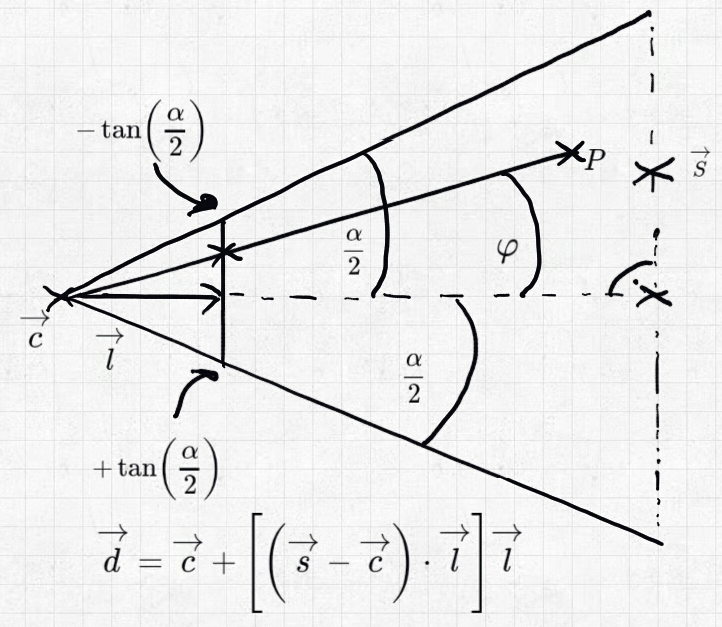
\includegraphics[width=0.5\textwidth]{perspective_image1}
\end{figure}

Display of point $P$ on screen:\newline
$X$/$Y$-Coordinates on screen for Point $P$ \newline
\centerline{$\boxed{ 2 \left(\dfrac{x - x_{0}}{screen-width/-height} - 0.5\right)\cdot tan \left(\dfrac{\alpha}{2}\right) = tan(\varphi)}$}
Where: 

$x_{0} =$ left Pixel

$w$ = screen width



\subsubsubsection{Zoom}
This approach to a zoom implementation does not use a change of the field of view (FoV) of the used camera, but simply works with changes in position of it. Instead of simply using the look at direction (camera front) and a preselected speed value, the formula used here defines a zoom factor and calculates a new position for the camera based thereon. If this zoom factor was set to the value $2$ for example, the camera would move to the position, where the whole image appears to be roughly two times the size of what it was before.

Per scroll-wheel rotation:

\begin{itemize}
	\item[]	Enlargement Factor $v$ (scroll backwards)
	\item[]	Enlargement Factor $\dfrac{1}{v}$ (scroll forwards)
	\item[]	Enlargement Factor after $r$ rotations: $v^{r}$ (The sign of $r$ result in the scroll direction)
\end{itemize}

\begin{itemize}
	\item[]	$\overrightarrow{c}_{old} = $ old camera position
	\item[]	$\overrightarrow{c}_{new} = $ new camera position
\end{itemize}
 \begin{table}[h!]
 	\begin{tabular}{p{5cm}p{6cm}}
 		$ v^{r} = \left(\dfrac{|\overrightarrow{c}_{new} - \overrightarrow{d}|}{|\overrightarrow{c}_{old} - \overrightarrow{d}| }\right)^{-1}$  &  \parbox[c]{2em}{ 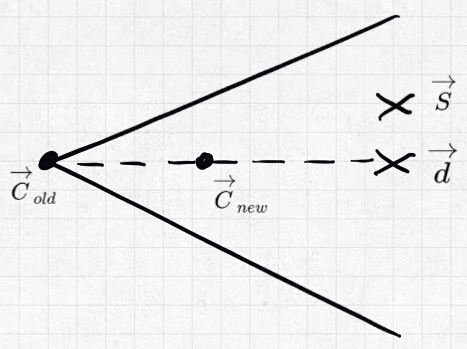
\includegraphics[width=1.5in]{perspective_image2} }\\
 		 &\\
 		$\Leftrightarrow  |\overrightarrow{c}_{new} - \overrightarrow{d}| = |\overrightarrow{c}_{old} - \overrightarrow{d}| \cdot v^{-r} $ & \\
 		$\overrightarrow{c}_{new} - \overrightarrow{d} ||\overrightarrow{c}_{old} - \overrightarrow{d} $ & \\
 		$\Leftrightarrow \boxed{\overrightarrow{c}_{new} =  \overrightarrow{d} + v^{-r}\left(\overrightarrow{c}_{old} - \overrightarrow{d}\right) }$  & \\
		& 		\centerline{\framebox[1.1\width]{Problem, if $\overrightarrow{c} = \overrightarrow{d}$ (corresponds to infinite enlargement)}} \par  \\
 	\end{tabular}
 \end{table}

\subsubsubsection{Shifting Motion (Hand-Movement)}
The theory behind this aspect of camera movement is for what is referred to as hand-movement in other applications and occurs when the user selects a pixel on the screen with the mouse cursor and then drags (mouse-key held down) the cursor a new pixel, on which he releases the key again.
This approach does not pay too much attention to the position calculated within the world-space with the \verb|readPixel| command, that uses the X- and Y-coordinates of a selected pixel on the screen. Instead it projects the two selected points onto the centre-plane mentioned above and then calculates the distance between those two values. This determined distance is then used to move the camera to a new position so whichever point the cursor was released on appears to have moved to the starting point of the executed dragging motion.


Shift Point with Coordinates $x$ to $x'$ \\

\noindent\textbf{Approach $a$:} \\
Formally correct shift of selected point based on the centre of the object it was located on. This approach only works if a point on any \gls{mesh} displayed within the scene (with $z > -1$) was selected and correctly identified by the \verb|readPixel| command. If that condition is not met, a fall-back to approach $b$ is required.

\begin{figure}[h!]
	\centering
	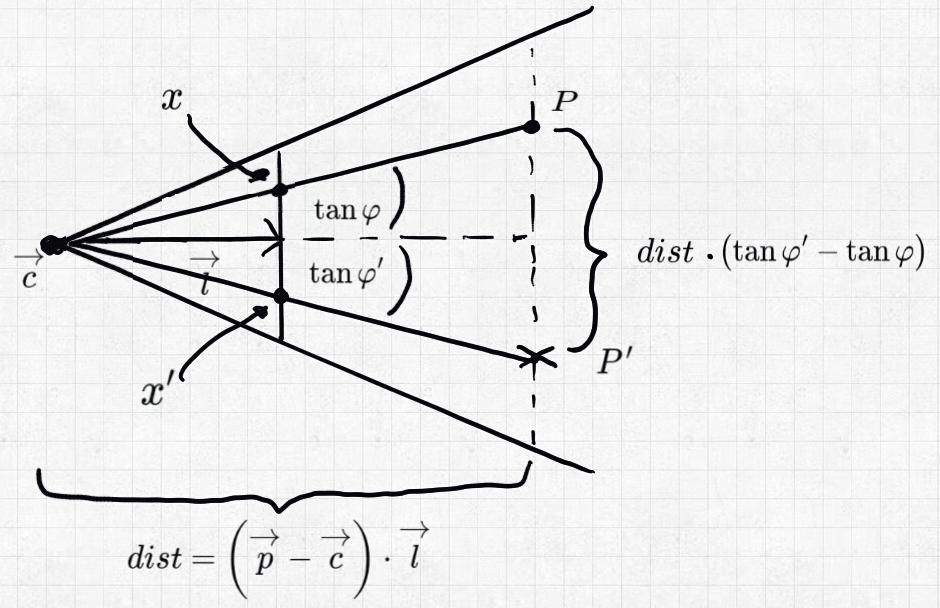
\includegraphics[width=0.5\textwidth]{perspective_image3}	
\end{figure}
$P$ Coordinates obtained via \verb|readPixel| function.	 
Shift of $P$ in x-Direction (world coordinates):

\begin{align*}\left(\overrightarrow{p} - \overrightarrow{c}\right)\overrightarrow{l} \cdot \left[2\left(\dfrac{x' - x_{0}}{w} - 0.5\right)tan\left(\dfrac{\alpha}{2}\right) - 2\left(\dfrac{x - x_{0}}{w} - 0.5\right)tan\left(\dfrac{\alpha}{2} \right)\right] = 2tan\left(\dfrac{\alpha}{2}\right)\left(\overrightarrow{p} - \overrightarrow{c}\right) \overrightarrow{l} \cdot \left(\dfrac{x' - x}{w} \right) 	\end{align*}

In vectorial form:                                                                                                                                                                                                                     

\begin{align*}  \Delta\overrightarrow{p} &= \dfrac{2tan\left(\dfrac{\alpha}{2}\right)\left(\overrightarrow{p} - \overrightarrow{c}\right) \overrightarrow{l}}{w} \cdot \underbrace{\left(\overrightarrow{p}'_{S} - \overrightarrow{p}_{S}\right)}_{ 
		\mathclap{\text{Screen Coordinates of $P'$ and $P$}}} \\                                                                                                                                                                                      \\ 
	\overrightarrow{c}_{new} &= \overrightarrow{c}_{old} -\Delta\overrightarrow{p}                                                                                                                                                                      
\end{align*}

Conversion of Screen Coordinates of $P'$ and $P$ in 3-D direction according to Camera Coordinate-System:

\begin{align*}
	& \overrightarrow{l} = \overrightarrow{l}_{z} & \overrightarrow{l}_{x} = \dfrac{\overrightarrow{l} \times \overrightarrow{n}}{|\overrightarrow{l}\times \overrightarrow{n}|} &   & \overrightarrow{l}_{y} = \overrightarrow{l}_{x} \times \overrightarrow{l}_{z} &   
\end{align*}

\noindent\textbf{Approach $b$:} \newline

This approach has the advantage of working with all points on the screen and not only for those on any given \gls{mesh}. It is based on a shifting velocity independent of the selected start and end points of the dragging motion, where the velocity is inverse proportional to the enlargement factor. 
This also results in the effect, that the mouse cursor ends up being inaccurate and therefore misleading for the user. This mouse-cursor issue can be avoided if the selected pixel is marked in the model, but the mouse cursor hidden afterwards. At operation's end the mouse cursor can be set back in the starting position using the \verb|SetCursor| command and the previously determined position. \newline


\begin{align*} 
	Modified:  dist &= \left( \overrightarrow{s} - \overrightarrow{c}_{old}\right) \cdot \overrightarrow{l} \\
	\Rightarrow \Delta\overrightarrow{p} &= \dfrac{2tan\left(\dfrac{\alpha}{2}\right)\left(\overrightarrow{s} - \overrightarrow{c}_{old}\right) \cdot \overrightarrow{l}}{w} \left(\overrightarrow{p}'_{s} - \overrightarrow{p}_{s} \right)  \\
	\\
	\overrightarrow{c}_{new} &= \overrightarrow{c}_{old} - \Delta \overrightarrow{p}
\end{align*}

\centerline{\framebox[1.1\width]{Problem, if $\overrightarrow{c}_{old}$  is located on the centre-plane (infinite enlargement $\mathrel{\widehat{=}}$ 0-shift factor)  }} \par  



\subsubsubsection{Rotations}
There are multiple concepts such as the \verb|arcball| available in order to perform a rotation within a scene based on a selected point. The approach we intend to use here is based around the $d$ axis also referred to as rotation centre within this chapter and uses a constant rotation velocity.
The potentially negative aspect of this approach for the user is, that the rotation performed after selecting an initial starting point can not be reliably connected to the mouse cursor. This is only be possible with a low rotation velocity, but appears to be more appealing when compared to the alternative of inconsistent speeds.

Assumption: the rotation around the pixel distance $\sqrt{\Delta x^{2} + \Delta y^{2}}$ is $\dfrac{\sqrt{\Delta x^{2} + \Delta y^{2}}}{w} \cdot \beta $ (f.e. $\beta = T_{0} $)

Rotation Axis: We divide the rotation in 2 parts:
\begin{itemize}
	\item[] Rotation of $\left(\dfrac{x}{y}\right)$ around the centre of the scene
	\item[] After that, rotation from the centre of the scene to $ \left(\dfrac{x'}{y'} \right)$
\end{itemize}

In both rotations the plane perpendicular to the rotation axis contains the points $\overrightarrow{c}$ and $\overrightarrow{d}$, and additionally either the point $ \overrightarrow{c} + \left(\begin{smallmatrix}tan (\alpha_{x}) \\ tan (\alpha_{y}) \\ 1\end{smallmatrix}\right) $ or $ \overrightarrow{c} + \left(\begin{smallmatrix}tan (\alpha_{x'}) \\ tan (\alpha_{y'}) \\ 1\end{smallmatrix}\right) $

The rotation axis is thus:
\begin{align*}
	& \overrightarrow{l} \times \left(\begin{smallmatrix}tan (\alpha_{x}) \\ tan (\alpha_{y}) \\ 1\end{smallmatrix}\right)  or   \overrightarrow{l} \times \left(\begin{smallmatrix}tan (\alpha_{x'}) \\ tan (\alpha_{y'}) \\ 1\end{smallmatrix}\right)  &  
\end{align*}

\noindent\textbf{Step 1}

$R_{1} = $ rotation around $\overrightarrow{d}$ with rotation axis   $\overrightarrow{l} \times \left(\begin{smallmatrix}tan (\alpha_{x}) \\ tan (\alpha_{y}) \\ 1\end{smallmatrix}\right)$ and rotation angle $\sqrt{x^{2} + y^{2}} \cdot \beta $

\noindent\textbf{Step 2}

$R_{2} = $ rotation around $\overrightarrow{d}$ with rotation axis   $\overrightarrow{l} \times \left(\begin{smallmatrix}tan (\alpha_{x'}) \\ tan (\alpha_{y'}) \\ 1\end{smallmatrix}\right)$ and rotation angle $- \sqrt{x^{2} + y^{2}} \cdot \beta $

\noindent\textbf{Step 3}

Rotation of $\overrightarrow{c}$ around $R_{1}R_{2}$ \newline
\indent Rotation of the \verb|lookAt| direction $\overrightarrow{l}$ around $R_{1}R_{2}$ \newline

\noindent Problems: 
Adjustment of near and far plane necessary: yes

The new $\overrightarrow{c}$-Value can coincide with $\overrightarrow{s}$ $\mathrel{\widehat{=}}$ Enlargement $\infty$ (shift $\overrightarrow{s}$ temporary)
 
\subsection{Testing} \label{testing}

\subsubsection{Cute Framework}

After trying several unit test frameworks we decided to employ the Cute Framework \cite{cute}, as we already had gathered experience with it in the C++ course at the HSR and the integration into the project offered the least complications.

Cute has no graphical support in Visual Studio, meaning that there is no "Green Bar". On the contrary, as command line framework, it even is possible to execute the tests without an instance of Visual Studio running, which is an advantage in most of cases.

The installation of Cute as standalone version is straight forward, as Cute is a "header library" and thereby only needs to have its header files included in the project.

\subsubsection{Testing Proceeding}

The \emph{Jaw Viewer} is mostly a graphical application with the primary goal of displaying objects on the screen. Because of this we decided to follow the Test Driven Development principles only for "testable" components, or components with a behaviour suited for unit and integration tests. The correctness of the displayed objects and movements was verified in the meetings by means of reviews by the Clinic, but due to the time loss described in \ref{reverse-engineering} Reverse Engineering, it was not feasible to realize usability tests during our project.

\subsubsection{Unit Tests}

The components of the \verb|common| package and some classes of the \verb|viewer| were developed under TDD principles. These components perform mathematical calculations, read files or perform other activities, which can be tested bythe  means of unit tests. In each case the equivalence partitioning and boundary-values testing approaches have been followed. 

Thanks the data provided by the Clinic the use of mocks could be avoided in this first implementation, always employing original values. An example of this is the \verb|mvm_file_parser_test_suite|, which tests the \verb|MvmFileManager| class. As a reminder, the \verb|MvmFileManager| reads a MVM file and extracts the coordinates saved in it to \glspl{frame}.

\noindent This suite ranges from very specific tests (check if the x LED coordinate is correct) all the way to integration tests in which we check whole blocks of coordinates are read and processed correctly.

As already mentioned, each component or class is tested with a test suite. The creation of a test suite in \verb|cute |is simple. First we declare the test suite header file:


\begin{lstlisting}[language=C++, caption=Test Suite header file]
#pragma once
#ifndef STL_FILE_PARSER_TEST_SUITE
#define STL_FILE_PARSER_TEST_SUITE

#include "cute_lib/cute_suite.h"

extern cute::suite make_suite_stl_file_parser_test_suite();

#endif
\end{lstlisting}

Each test suite must test only one class or struct and then be registered into Cute:

\begin{lstlisting}[language=C++, caption=Test Suite registration]
// ViewerTest.cpp : Defines the entry point for the console application.

#include "stdafx.h"
#include "cute_lib/cute.h"
#include "cute_lib/ide_listener.h"
#include "cute_lib/xml_listener.h"
#include "cute_lib/cute_runner.h"
#include <iostream>

#include "stl_file_parser_test_suite.h"

bool runSuite(int argc, char const* argv[]) {
	using namespace std;
	cute::xml_file_opener xmlfile(argc, argv);
	cute::xml_listener<cute::ide_listener<>> lis(xmlfile.out);

	auto runner = cute::makeRunner(lis, argc, argv);
	auto stlFileParserTestSuite{make_suite_stl_file_parser_test_suite()};

	auto success = runner(stlFileParserTestSuite, "STL_FILE_PARSER_TEST_SUITE");
	std::cin.get();
	return success;
}

int main(int argc, char const* argv[]) {
	return runSuite(argc, argv) ? EXIT_SUCCESS : EXIT_FAILURE;
}
\end{lstlisting}

And finally we write the unit test in the test suite source file:
\begin{lstlisting}[language=C++, caption=Test Suite unit tests]
#include "stdafx.h"
#include "stl_file_parser_test_suite.h"
#include "cute_lib/cute.h"
#include "../common/stl_parser.h"

void test_file_no_exists_exception() {
	stl::StlFileManager manager{};
	ASSERT_THROWS(manager.parse_stl_file("foo"), std::logic_error);
}

cute::suite make_suite_stl_file_parser_test_suite() {
	cute::suite s{};
	s.push_back(CUTE(test_file_no_exists_exception));
	return s;
}
\end{lstlisting}


\subsection{Dependencies}

\subsubsection{OpenGL Dependencies}

As already mentioned in \ref{opengl-profiles} Core and Compatibility Profiles, we develop this project with OpenGL core profile, version 3.3. This is due first because the tutorial \cite{learnopengl} the project bases on is written with the 3.3 version, and also in order to support "not state of the art" hardware. 
Higher versions of OpenGL (current 4.5) are not supported by older hardware. Despite of OpenGL's backwards compatibility, it's proven \cite{superbible} that not all hardware supports all new features of newer versions of OpenGL. Therefore we decided to remain by the given 3.3 OpenGL version.	

\subsubsection{C++ Dependencies}

A project goal was the use of the least possible number of external libraries, and less in other programming languages. In other words, the project shall remain pure C++ and C\#.

\begin{itemize}
	\item[] \textbf{glfw} \cite{glfw} C++ Library for \gls{opengl}. It provides a simple, platform-independent API for creating windows, contexts and surfaces, reading input, handling events, etc.
	\item[] \textbf{glew} \cite{glew} Cross-platform open-source C/C++ extension loading library. Run-time mechanisms for determining which OpenGL extensions are supported on the target platform
	\item[] \textbf{glm} \cite{glm} Mathematics library for graphics software based on the \gls{glsl} specifications
	\item[] \textbf{jsoncpp} \cite{jsoncpp} C++ library for \verb|json| management
	\item[]	\textbf{cute} \cite{cute} C++ Testing Framework. Refer to \ref{testing} Testing
\end{itemize}


\subsection{Code Statistics}


The code lines were counted with Cloc \cite{cloc}. The lines quantity contains only self written code. External libraries were excluded.


\begin{table}[h!] 
	\begin{center}
		\begin{tabular}{ p{2.3cm}||p{1cm}|p{1cm}|p{1.4cm} |p{1cm} }\beforeheading
			\heading{\textbf{Language}} & \heading{\textbf{Files} }   & \heading{\textbf{code}}	\\\afterheading
			C++  			      		& 22             			  & 6264					\\\normalline
			C++ Header                  & 29                          & 672              		\\\normalline
			GLSL		                & 2                           & 44              		\\\normalline
			C\#	 	          	 	    & 14                          & 1670          			\\\lastline
			\textbf{Total}  	 	    & 67		                  & 8650 		            \\\lastline
		\end{tabular}
		\caption{Code Statistics}
	\end{center}
\end{table}

\noindent As already mentioned in \ref{testing} Testing, one of the disadvantages of \verb|cute| is being a command line framework and the absence of integration in Visual Studio. This fact and the lack of code coverage tools in Visual Studio for C++ using this form of testing prevent us from showing code coverage statistics for this project.


\subsection{Results}

We can divide the results of this bachelor thesis in \textbf{Software} and in \textbf{Documentation}. 
The \textbf{Software} consists logically on the \emph{Jaw Viewer}, an application which fulfils the Use Cases 01 to 05 (see \ref{use-cases} Use Cases). 

\begin{figure}[h!]
	\centering
	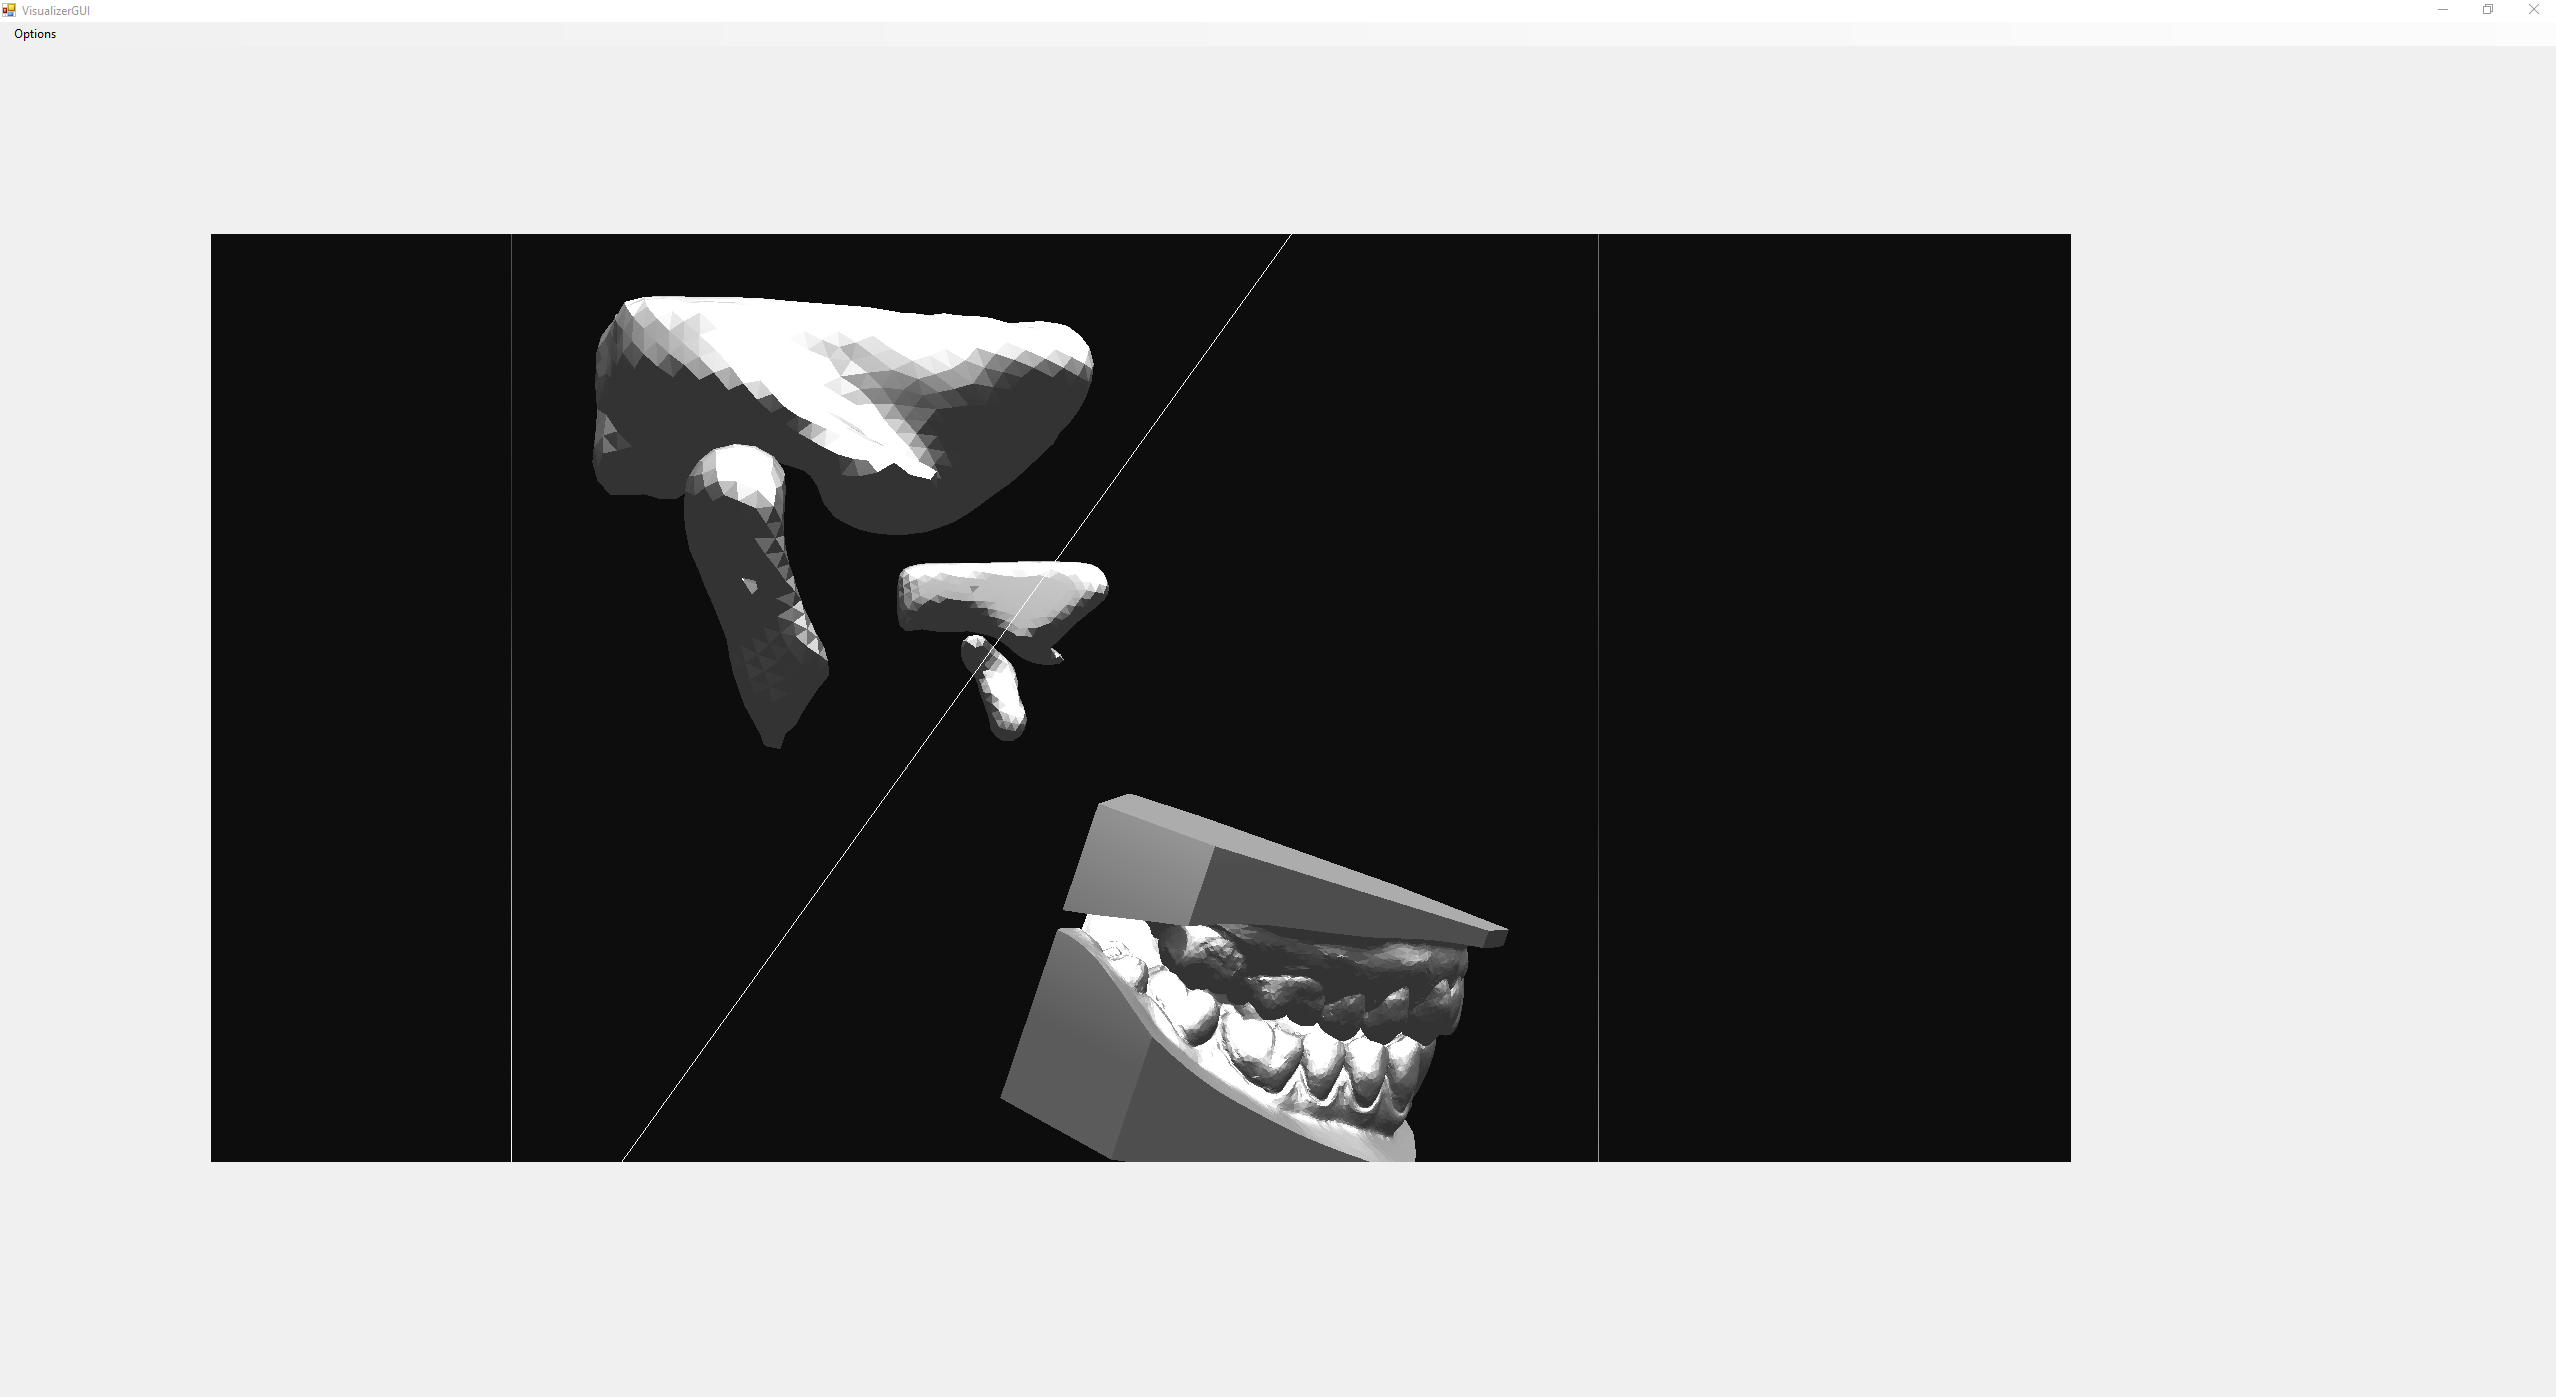
\includegraphics[width=1\textwidth]{jaw_viewer_gui}
	\caption{Jaw Viewer}
\end{figure}

\noindent This means that \emph{Jaw Viewer} is an application capable of:
\begin{itemize}
	\item Importing and processing \gls{STL} and \gls{MVM} files
	\item Configuring the movement and applying it to selected \gls{anatomy}
	\item Displaying the Anatomy Objects with and without movement (animation)
	\item Loading and saving the configuration for the application
\end{itemize}

\noindent But not all news are good. The Use Cases \ref{uc:6} Display anatomy movement in real time and \ref{uc:7} Save anatomy movement in real time could not be implemented within the time frame. During the different meetings with the Clinic, it became obvious that there was a discrepancy about the necessity of this initial requirement for this project, but also various other aspects. For some of the involved members of the Clinic that was a "must have" requirement as stated in the projects definition, whereas for others it was not. In the meeting after the interim presentation (on the 11th April 2017) the Clinic has agreed to making the real time features not imperative, allowing us to focus on the more basic challenges.

This discrepancy about the requirements was prevalent during the whole project. The meetings often resulted in more scattered requirements (often not specified in the initial project description) and confusion instead of useful and concrete information or instructions. This, combined with our lack of experience in this complex domain as well as handling clients in general, led to a point where we felt forced to distance us from the Clinic and focus on implementing as much as we could. Even if that meant searching for information the client should have provided us with and potentially finding alternative solutions to the challenges occurring.

In \ref{reverse-engineering} Reverse Engineering we described our attempts in order to find the correct transformation needed for the accurate display of the recorded movement for the \glspl{anatomy}. As already mentioned, due to the inconsistent and unclear information from the Clinic we could not reach this goal. This has led to the situation where although the \emph{Jaw Viewer} fulfills the use cases mentioned above, it is not ready for use in a productive environment. The displayed movement is not accurate enough and as such unreliable for a good diagnosis for patients.

On the bright side, the application together with the explanations therein can be considered a good base for future development in the same area. All the functionality and most importantly the data structures are already implemented. As such, they could be directly used, although they are subject to another refactoring process and of course a correction of the movement calculations. \newline

This \textbf{report}, as the other product of this bachelor thesis, can be considered an important documentation foundation for future projects in the same field. When we started the project there was next to no documentation of the proprietary software used by the Clinic (\gls{optis} and \gls{tmjviewer}), the used coordinate systems and the mathematical theories needed for this specific usage of \gls{opengl} for the dental medicine. With this report, any future developers tasked with the same can save a lot of time in the analysis stage while avoiding the undesired trial and error process we went through. Starting with this gathered information and from a fitting code structure should also allow them to concentrate on the more important and well identified tasks needed to actually create an alternative to the proprietary software currently in use.
